The Displacement-based Earthquake Loss Assessment (DBELA) methodology builds upon the urban assessment methodology proposed by \cite{Calvi1999}, in which the principles of structural mechanics and seismic response of buildings are used to estimate the seismic vulnerability of classes of buildings. The current implementation of the RMTK is only compatible with bare or infilled frame reinforced concrete structures.\\

In this method, the displacement capacity and demand for a number of limit states needs to be calculated. Each limit state marks the threshold between the levels of damage that a building might withstand, usually described by a reduction in strength or by exceedance of certain displacement/drift levels. Once these parameters are obtained, the displacement capacity of the first limit state is compared with the respective demand. If the demand exceeds the capacity, the next limit states need to be checked successively, until the demand no longer exceeds the capacity and the building damage state can be defined. If the demand also exceeds the capacity of the last limit state, the building is assumed to have collapsed. This procedure is schematically depicted in Figure \ref{fig:DBELA_scheme}, in which the capacities for three limit states are represented by $\Delta_i$ and the associated demand by $Sd_i$. In this example, the demand exceeds the capacity in the first and second limit state but not in the third limit state, thus allocating the building to the third damage state.

\begin{figure}[htb]
  \centering
      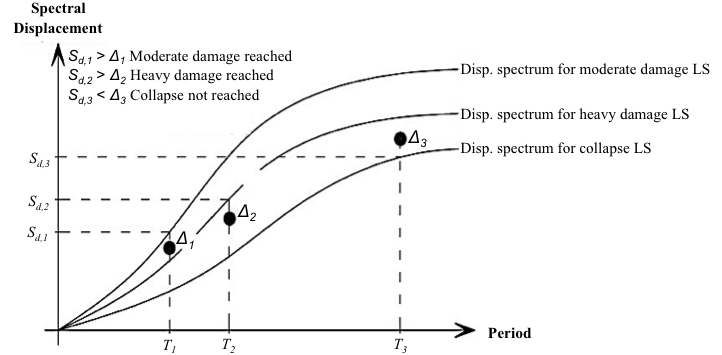
\includegraphics[width=12cm]{Figures/DBELA_scheme.png}
  \caption{Comparison between limit state capacity and the associated demand (adapted from \cite{BalEtAl2010}).}
  \label{fig:DBELA_scheme}
\end{figure}

The calculation of the displacement capacity at each limit state is explained in the Model Generation Section (\ref{sec:model-gen}), as this methodology can be employed to generate large sets of capacity curves (Sa versus Sd), which can be combined with other methodologies besides DBELA to derive fragility functions. Instead, this section is focused on describing how the seismic demand is handled in this methodology.\\ 

The demand is represented by a displacement spectrum which can be described as the expected displacement induced by an earthquake on a single-degree-of-freedom (SDOF) oscillator with a given period of vibration and viscous damping. This demand is initially calculated for a 5\% viscous damping, and later modified for each limit state using a correction factor ($\eta$), representative of the equivalent viscous damping and ductility at the associated damage state. In the Eurocode 8 \citep{CEN2005}, the following equation is proposed for the calculation of the correction factor:

\begin{equation}
\eta_{LS_i} = \sqrt{\frac{10}{5+\xi_{eq_i}}}
\end{equation}

Where $\xi_{eq_i}$ stands for the equivalent viscous damping at the limit state $i$. Although in theory there is a multitude of damping models in the literature that could be used to calculate this equivalent viscous damping (see Section \ref{subsec:CSM} for a description of the damping models implemented within the Capacity Spectrum Method), this method has been tested following the proposals by \cite{PriestleyEtAl2007} for reinforced concrete frames (e.g. \cite{BalEtAl2010} \cite{SilvaEtAl2013}). This model uses the following equation: 

\begin{equation}
\xi_{eq} = 0.05 + 0.565\left(\frac{\mu-1}{\pi\mu}\right)
\end{equation}
Where $\mu_i$ stands for the ductility at the limit state $i$ (assumed as the ratio between $\Delta_i$ and $\Delta_y$). More accurate approaches have recently been proposed to estimate the correction factors ($\eta$), considering additional parameters, such as the magnitude or source-to-site distance \citep{RezaeianEtAl2012}.\\
With regards to the calculation of the yielding period ($T_y$) for bare frame structures, \cite{CrowleyPinho2004} and \cite{CrowleyEtAl2008} proposed a relationship between the period and the total height ($H_T$) of $0.10H_T$ and $0.07H_T$ for structures without and with lateral load design, respectively. For infilled frames, a relation equal to $0.06H_T$ has been recommended by \cite{CrowleyPinho2006} for structures without lateral load design. The elongated period of vibration for any of the limit states ($T_{LS_i}$) can be computed using the following formula:
\begin{equation}
T_{LS_i} = T_y\sqrt{\frac{\mu_{i}}{1+\alpha\mu_{i}-\alpha}}
\end{equation}
where $\alpha$ stands for the post-yield stiffness ratio. In cases where this ratio can be assumed as zero, the relation between $T_{LS_i}$ and $T_y$ will depend purely on the limit state ductility as follows:

\begin{equation}
T_{LS_i} = T_y\sqrt{\mu_{i}}
\end{equation}

In order to use this methodology, it is necessary to first assess the capacity displacement of one or multiple assets, following the DBELA approch explained in Section \ref{subsec:DBELA} (Model Generator). Moreover, a set of ground motion records and a damage model should be provided, as explained in Section \ref{subsec:gmrs} and \ref{subsec:dmg_model}), respectively. The type of structures that are being evaluated should be specified using the parameter \verb=structure_type=. Currently this module of the RMTK accepts the options \verb=bare frame= and \verb=infilled frame=. After importing the module \verb=DBELA=, it is possible to calculate the distribution of structures across the set of damage states for each ground motion record using the following command:

\begin{Verbatim}[frame=single, commandchars=\\\{\}, samepage=true]
PDM, Sds = DBELA.calculate_fragility(capacity_curves,gmrs,...
damage_model,structure_type)
\end{Verbatim}

Where \verb=PDM= (i.e. probability damage matrix) represents a matrix with the number of structures in each damage state per ground motion record, and \verb=Sds= (i.e. spectral displacements) represents a matrix with the maximum displacement (of the equivalent SDOF) of each structure per ground motion record. the variable PDM can then be used to calculate the mean fragility model as described in Section \ref{subsec:derive_fragility}.